\chapter{Quantum Dot Results}

\section{One Dimension}

\subsection*{Four electrons}

\begin{figure}[h]
    \centering
    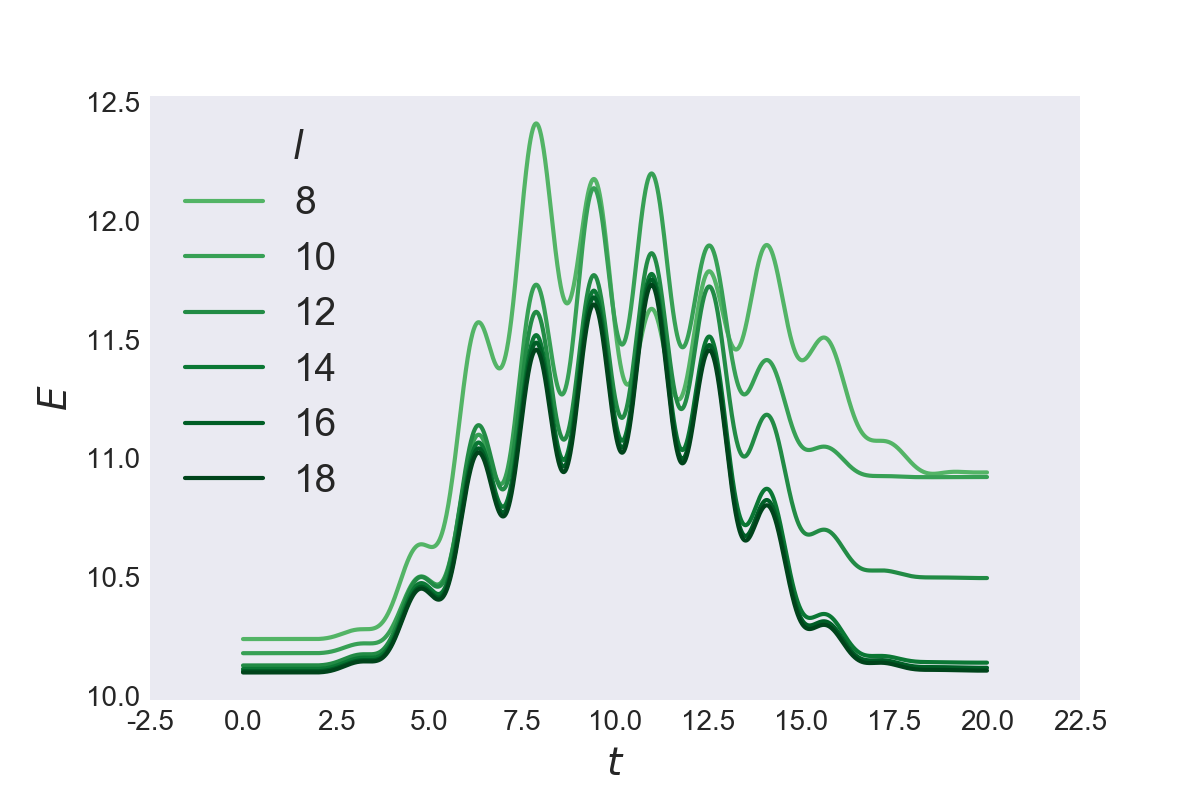
\includegraphics[width=0.75\textwidth]{results/figures/1D/n=4energy.png} 
    \caption{Time-dependent energy of a one-dimensional harmonic oscillator with $\Omega=1$
        and $n=4$ electrons under the influence of a oscillating electric field 
        of frequency $\omega = 2 \Omega = 2$ and field strength $E=1$, for 
        different number of spin-orbitals $=\{8,10,12,14,16,18\}$.
    }
    \label{fig:1d_n4_qd}
\end{figure}

\pagebreak

\subsection*{Six electrons}

\begin{figure}[!h]
    \centering
    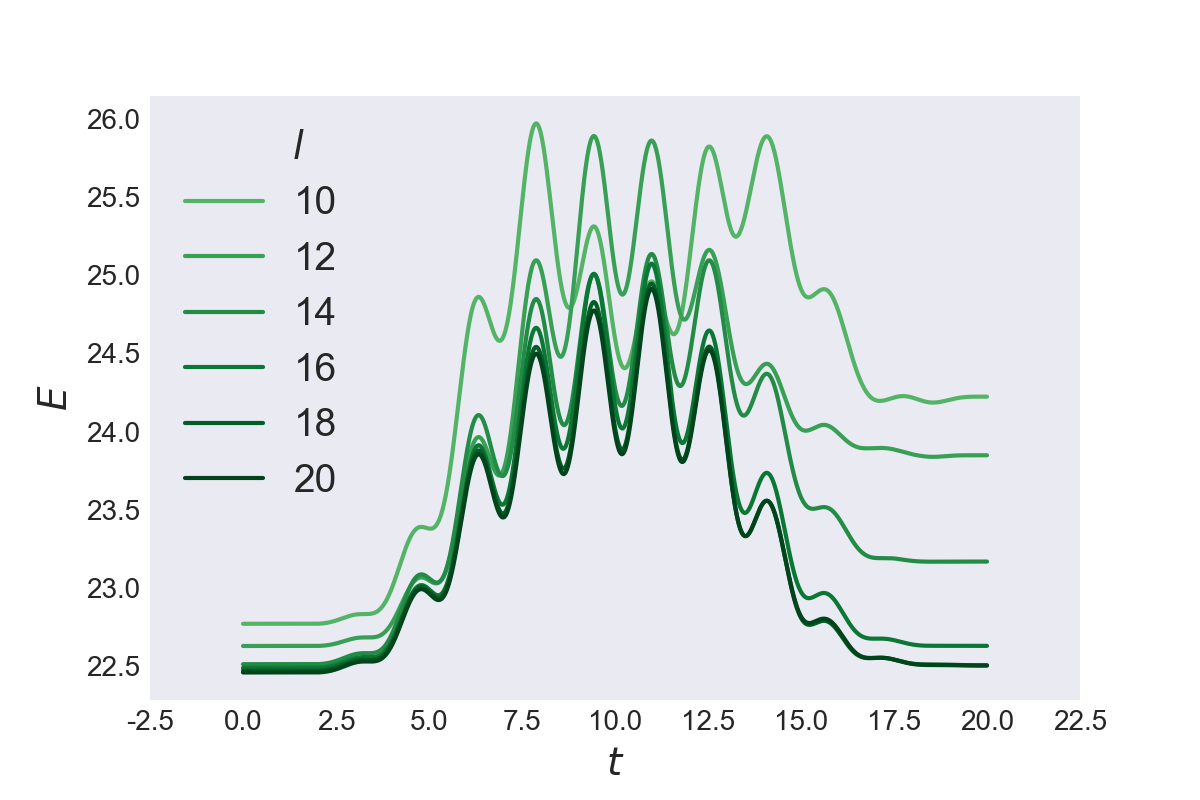
\includegraphics[width=0.75\textwidth]{results/figures/1D/n=6energy.png} 
    \caption{Time-dependent energy of a one-dimensional harmonic oscillator with $\Omega=1$
        and $n=6$ electrons under the influence of a oscillating electric field 
        of frequency $\omega = 2 \Omega = 2$ and field strength $E=1$, for different 
        number of spin-orbitals $l=\{10,12,14,16,18,20\}$.
    }
    \label{fig:1d_n6_qd}
\end{figure}

\subsection*{Eight electrons}

\begin{figure}[!h]
    \centering
    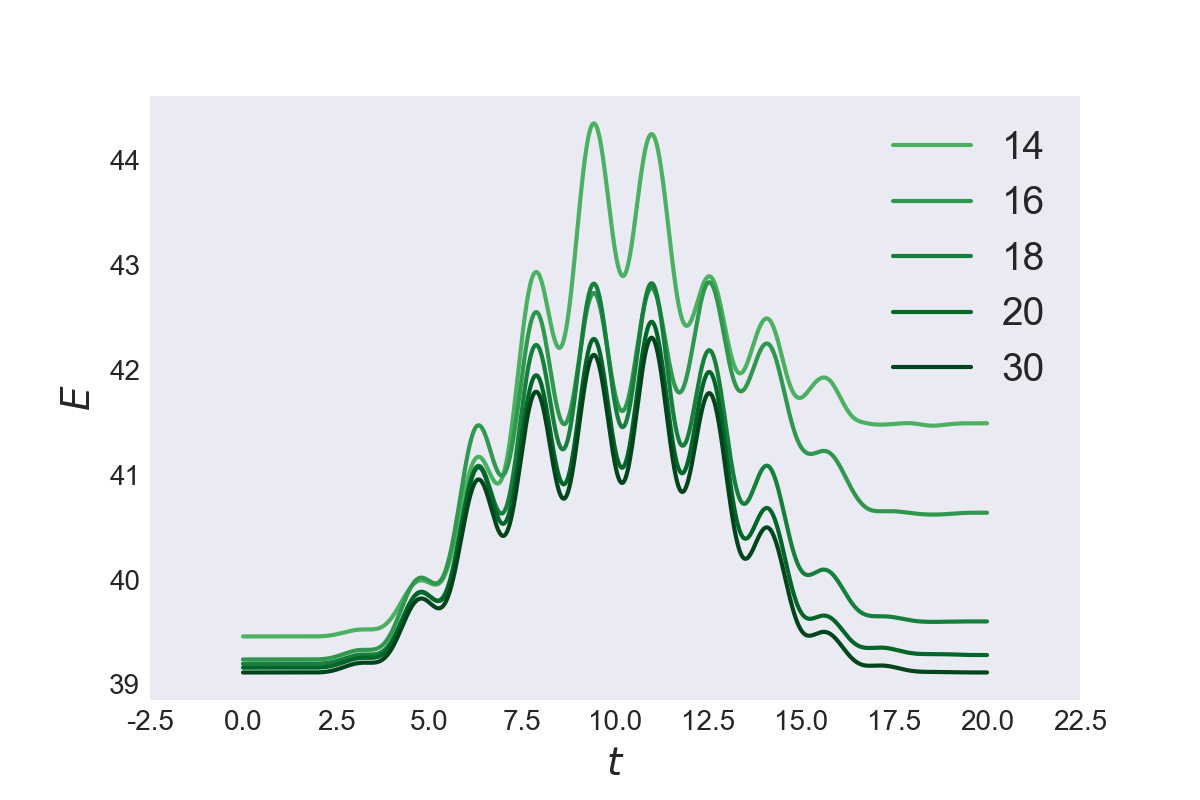
\includegraphics[width=0.75\textwidth]{results/figures/1D/n=8energy.png} 
    \caption{Time-dependent energy of a one-dimensional harmonic oscillator with $\Omega=1$
        and $n=8$ electrons under the influence of a oscillating electric field 
        of frequency $\omega = 2 \Omega = 2$ and field strength $E=1$, for different 
        number of spin-orbitals $l=\{14,16,18,20,30\}$.
    }
    \label{fig:1d_n8_qd}
\end{figure}

\pagebreak

\subsection*{Ten electrons}

\begin{figure}[!h]
    \centering
    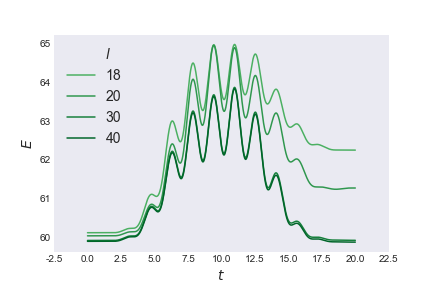
\includegraphics[width=0.75\textwidth]{results/figures/1D/n=10energy.png} 
    \caption{Time-dependent energy of a one-dimensional harmonic oscillator with $\Omega=1$
        and $n=10$ electrons under the influence of a oscillating electric field 
        of frequency $\omega = 2 \Omega = 2$ and field strength $E=1$, for different 
        number of spin-orbitals $l\{18,20,30,40\}$.
    }
    \label{fig:1d_n10_qd}
\end{figure}

\subsection*{Twelve electrons}

\begin{figure}[!h]
    \centering
    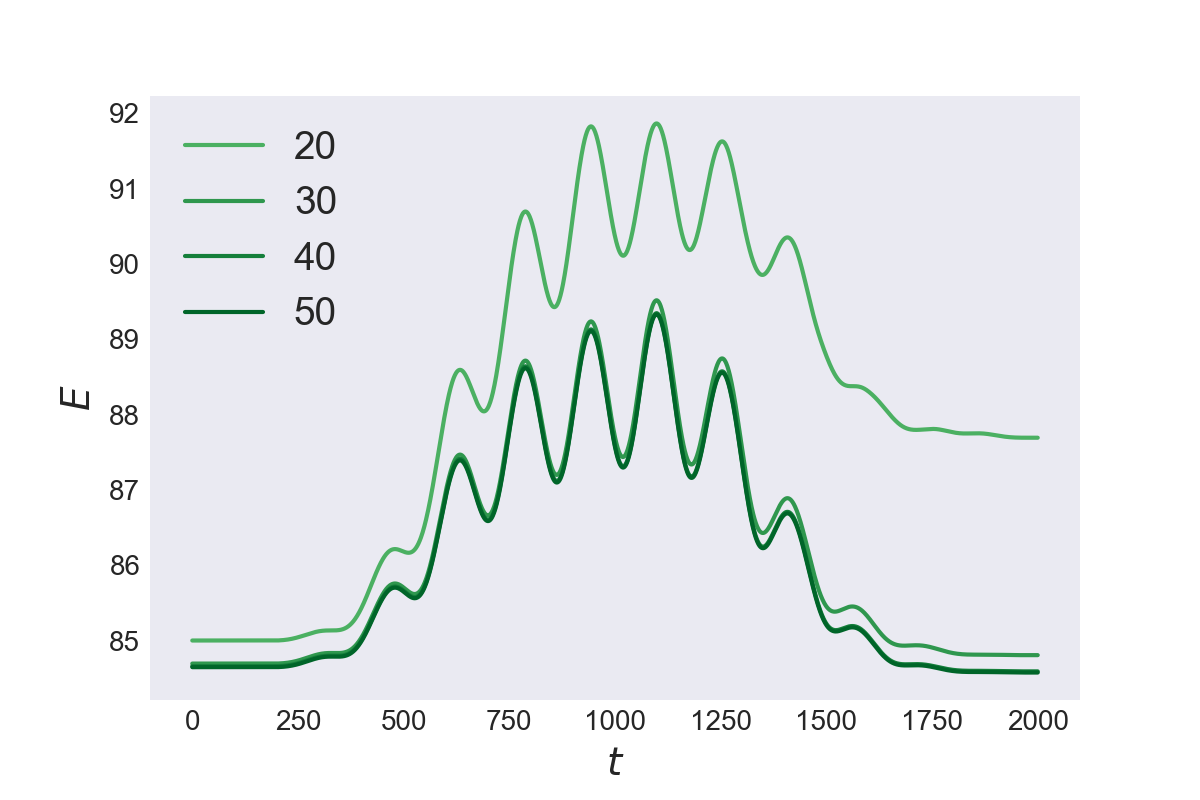
\includegraphics[width=0.75\textwidth]{results/figures/1D/n=12energy.png} 
    \caption{Time-dependent energy of a one-dimensional harmonic oscillator with $\Omega=1$
        and $n=12$ electrons under the influence of a oscillating electric field 
        of frequency $\omega = 2 \Omega = 2$ and field strength $E=1$, for different 
        number of spin-orbitals $l=\{20,30,40,50\}$.
    }
    \label{fig:1d_n12_qd}
\end{figure}